% !BIB TS-program = biber
\documentclass[man]{apa6}

\usepackage[style=apa,sortcites=true,sorting=nyt,backend=biber]{biblatex}

\DeclareLanguageMapping{american}{american-apa}

\addbibresource{refs.bib}

\title{Signal Detection Theory with Ambivalent or Missing Responses}

\shorttitle{SDT with ambivalent responses}

\author{Samuel R. Mathias, Emma E. E. M. Knowles, and David C. Glahn}

\affiliation{Yale University}

\abstract{Signal detection theory (SDT) allows researchers to calculate psychologically meaningful measures from behavioral data, so long as the design of the experiment conforms to one of the traditional SDT paradigms. These paradigms usually require subjects to make an affirmative response (e.g., ``yes'' or ``no'') to each trial. Occasionally, researchers may wish to allow subjects to make ambivalent responses (e.g., ``I don't know''), or not force them to respond to all trials. Here, we propose modifications to the standard SDT models that allow ambivalence and omissions for yes-no and two-alternative forced-choice experiments. Under these models, the equations for calculating sensitivity ($d^\prime$) are the same as those of regular SDT, but the equations for response bias ($c$) are different. Furthermore, we derive two new psychologically meaningful measures we call ``indices of uncertainty,'' $u$ and $u^\prime$, that allow researchers to quantify subjects' ambivalence.}

\keywords{signal detection theory, methods, modeling, statistics}
\authornote{Samuel R. Mathias, Department of Psychiatry, Yale School of Medicine, Yale University, New Haven, Connecticut; Emma E. E. M. Knowles, Department of Psychiatry, Yale School of Medicine, Yale University, New Haven, Connecticut; David C. Glahn, Department of Psychiatry, Yale School of Medicine, Yale University, New Haven, Connecticut.

This work was supported in part by grants from the National Institute of Mental Health.

Correspondence concerning this article should be addressed to Samuel R. Mathias, Suite 3014, 2 Church Street South
New Haven, CT 06519. E-mail:~samuel.mathias@yale.edu}

\begin{document}

\maketitle

\section{Introduction}
Signal detection theory is a widely used framework that allows researchers to transform the raw data from an experiment---the counts of trials and responses---into psychologically meaningful measures of sensitivity and bias. Methods for calculating these measures are generally straightforward to implement for common experimental designs \parencite[see][]{Green1966, Macmillan2005}. The two most common designs are yes-no (YN) and two-alternative forced-choice (2AFC).

In most experiments with SDT-friendly designs, subjects are required make an affirmative response (e.g., ``yes'' or ``no;'' ``first'' or ``second'') to each trial. However, researchers occasionally may wish to conduct experiments that do not require affirmative responses. For example, the standard YN and 2AFC designs could be modified to include an additional response that allows subjects to indicate ambivalence towards the other responses (e.g. ``I don't know''). However, including ambivalent responses flouts the requirements of regular SDT models, making it less straightforward to calculate sensitivity and bias.

Consider the recent study by \textcite{laskowskaemotional2015}, in which patients with Parkinson's disease, patients with schizophrenia, and healthy controls completed a test of facial emotion recognition. On each trial, subjects saw a photograph of a face and reported which of six possible emotions were conveyed, and which were not, by choosing one of three possibilities per emotion: ``shown,'' ``not shown,'' and ``hard to say.'' It was possible for a photograph to display more than one emotion. The authors analyzed the data using a standard SDT model by considering each response (six per photograph) as a separate YN trial. The authors found that, on average, the Parkinson's disease and schizophrenia patients had lower sensitivity to facial emotions than the controls, and that the Parkinson's disease patients adopted a more liberal response strategy than the controls. However, the authors had to recode ``hard to say'' responses before they could calculate sensitivity and bias, which vitiates the interpretation of their statistically significant group differences.

Other examples of experiments that do not conform to the requirements of regular SDT models can be found in the neuroimaging literature, where subjects are often required to perform specific tasks while their brain activity is recorded. Such experiments typically require strict control over the time intervals between trials and cannot guarantee that subjects will respond in time to every trial. In the functional magnetic resonance imaging (fMRI) study by \textcite{kreitewolfhemispheric2014}, subjects performed two tasks. In one task, subjects heard sequences of words, and indicated whether each word was the same as or different to the word that preceded it. In the other task, subjects heard the same sequences, and indicated whether sequential words had the same or a different intonation (either rising or flat). The researchers were primarily interested in differences in brain activity related to phonological and lexical processing; therefore, to compensate for differences related to task difficulty, subjects' percent correct scores were used as covariates in the fMRI analysis. Missing responses were simply labelled as incorrect. Under these circumstances, SDT measures of sensitivity and bias might have been better covariates than percent correct.

In the present paper, we present a method for dealing with ambivalent or missing responses in YN and 2AFC experiments. This method involves modifying regular SDT models, and re-deriving the equations for estimating sensitivity and bias. We show that, for both YN and 2AFC experiments, the equations for estimating sensitivity are actually the same as those of the regular SDT models, but the equations for estimating bias are different. Furthermore, our modified models also allow a new psychologically meaningful SDT measure to be estimated from the data. We call this measure the ``index of uncertainty'' because it reflects the degree of uncertainty or ambivalence within the decision process. We performed simulations to test the utility of our models in practice, and examined how previously used recoding strategies \parencite[e.g.,][]{laskowskaemotional2015, kreitewolfhemispheric2014} effect the estimates of SDT measures.

\section{SDT models}
\subsection{Regular YN model}
The \emph{equal-variance Gaussian SDT model for YN experiments}, hereby referred to as the regular YN model, was the first SDT model to be described \parencite{Peterson1954, Tanner1954} and forms the foundation of all SDT analysis. It has been outlined in detail by many previous authors \parencite[e.g.,][]{Green1966, Macmillan2005}. We outline it again briefly here, so that readers can see the difference between this model and our modified version, described later on.

Under the model, each trial of the experiment contains a single stimulus drawn at random from one of two classes, and the subject indicates to which class the stimulus belonged. Let $X$ represent the stimulus class. When $X=0$, the stimulus is drawn from the first class, and when $X=1$, the stimulus is drawn from the second class. The model assumes that the subject generates a random variable (or ``observation'') from the stimulus. These observations are denoted $\Psi$. If $X=0$, $\Psi$ has a standard normal probability distribution, $\Psi_{X=0}\sim{}\mathcal{N}\left(0,1\right)$. If $X=1$, $\Psi$ has a normal probability distribution with mean $d$ and unit standard deviation,
$\Psi_{X=1}\sim{}\mathcal{N}\left(d,1\right)$. When $d$ is large, the two distributions are distinct, and the subject can easily distinguish between the stimulus classes. If $d=0$, the classes are indistinguishable. Thus, $d$ is a measure of sensitivity\footnote{In the literature, the more commonly used index of sensitivity is $d^\prime$, where the $^\prime$ symbol represents the fact that the distance between the means of the two distributions of observations is ``standardized''  (i.e., $d$ divided by the pooled standard deviation). However, since we assume here that the standard deviations of both distributions are 1, there is actually no difference between $d$ and $d^\prime$. The distinction between $d$ and $d^\prime$ becomes important when either standard deviation is not set to 1, such as in unequal-variance SDT models.}

Let $Y$ represent the subject's response to a trial. When $Y=0$, the subject responds that the stimulus was in the first class, and when $Y=1$, the subject responds that the stimulus was in the second class. Under the model, the subject makes a response based on whether $\Psi$ is smaller or greater than some fixed threshold (or ``criterion''), denoted $k$. Formally, this decision rule can be written
\begin{eqnarray*}
&Y=0\textrm{ if }\Psi<k\textrm{,}\\
&Y=1\textrm{ if }\Psi\ge{}k\textrm{.}
\end{eqnarray*}When $k=\frac{d}{2}$, the subject is said to be ``unbiased,'' since both responses are equally likely. The distance between true $k$ and unbiased $k$ is denoted $c$. Thus, $c$ is a measure of bias.

The model is summarized in the left panel of Fig.~\ref{fig:Figure1}. The figure shows two important additional variables. The blue shaded region represents the probability of a ``false alarm,'' that is, when $Y=1$ given $X=0$. We denote this probability $f$. The green shaded region represents the probability of a ``hit,'' that is, when $Y=1$ given $X=1$, denoted $h$. These conditional probabilities can be expressed in terms of $d$ and $c$:
\begin{eqnarray*}
P\left\{Y=1\mid{}X=0\right\}=f&=&1-\Phi\left(k\right)\\
&=&1-\Phi\left(c+\frac{d}{2}\right)\textrm{,}
\end{eqnarray*}where $\Phi\left(.\right)$ denotes the standard normal cumulative distribution function; and
\begin{eqnarray*}
P\left\{Y=1\mid{}X=1\right\}=h&=&1-\Phi\left(k-d\right)\\
&=&1-\Phi\left(c-\frac{d}{2}\right)\textrm{.}
\end{eqnarray*}

\begin{figure}
    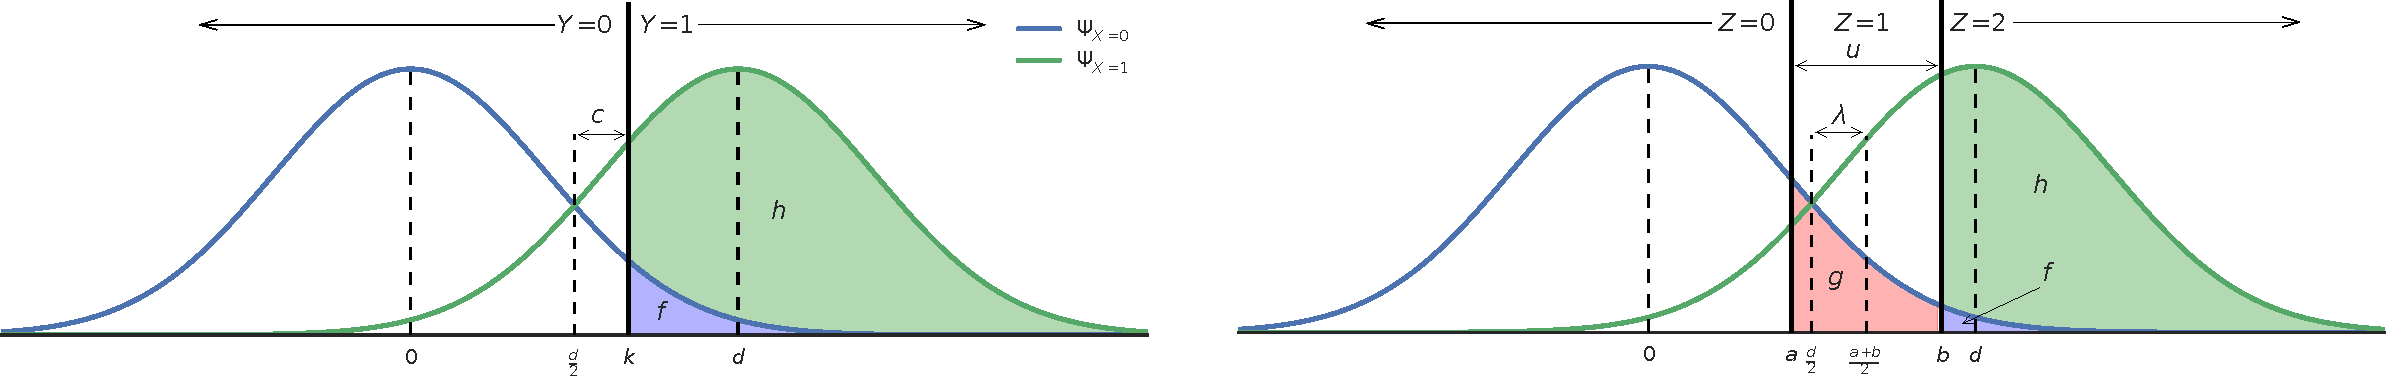
\includegraphics[width=1\textwidth]{Fig1_4.pdf}
    \caption{Illustrations of the regular YN model (left panel) and the modified YN model (right panel). In both panels, the two curves represent the probability distributions of observations from the two stimulus classes. Under the regular model, the distance between the means of the distributions, $d$, is a measure of sensitivity, and the distance between $\frac{d}{2}$ and $k$, denoted $c$, is a measure of bias. Both of these measures can be expressed uniquely in terms of the false-alarm and hit probabilities ($f$ and $h$, respectively). Under the modified model, $d$ is again an appropriate measure of sensitivity and can be estimated in the same way. However, an appropriate measure of bias, $\lambda$, is calculated differently, and requires an additional probability, $g$, to be estimated from the data. The modified model contains an additional measure, $u$, that represents uncertainty or ambivalence in the decision process.}
    \label{fig:Figure1}
\end{figure}

Crucially, because $f$ and $h$ can be estimated directly from the data in an experiment, the above equations can be combined and re-arranged to produce estimates of sensitivity and bias. Specifically, the equation for estimating sensitivity is
\begin{eqnarray}
\hat{d}&=&\Phi^{-1}\left(\hat{h}\right)-\Phi^{-1}\left(\hat{f}\right)\textrm{,}
\label{eq1}
\end{eqnarray}where $\Phi^{-1}\left(.\right)$ denotes the probit function, and a caret denotes the \emph{maximum-likelihood estimate} of a variable. The equation for estimating bias is
\begin{eqnarray}
\hat{c}&=&-\frac{1}{2}\left[\Phi^{-1}\left(\hat{h}\right)+\Phi^{-1}\left(\hat{f}\right)\right]\textrm{.}
\label{eq2}
\end{eqnarray}

It is worth noting that the assumptions of the regular YN model can be relaxed in various ways. For example, it is possible for the probability distributions of $\Psi_{X=0}$ and $\Psi_{X=1}$ to be non-Gaussian, or have different variances. Indeed, work on recognition memory has consistently reported phenomena that are inconsistent with the regular YN model but can be explained by assuming unequal variances \parencite{Wixted2007, Yonelinas2007} or by assuming that $\Psi_{X=0}$ and $\Psi_{X=1}$ are drawn from mixtures of latent distributions \parencite{decarlosignal2002}. Another possibility is to allow $k$ to vary across trials rather than remaining constant over trials \parencite{cabreraseparating2015}. However, relaxing any of these assumptions means that the YN model is no longer exactly identified (i.e., the number of independent unknown variables and the number of known variables are not the same), so consequently cannot be solved for $d$ and $c$. For the purposes of this article, we adhere to these assumptions, but note that future work could extend our models to incorporate unequal variance, non-Gaussian decision variables, and variable criteria.

\subsection{YN model with ambivalent or missing responses}
One can account for ambivalent or missing responses with two modifications to the regular YN model, as shown in the right panel of Fig.~\ref{fig:Figure1}. The first modification is that the model contains two criteria, denoted $a$ and $b$. The second modification is to the decision rule. Let $Z$ denote the subject's response. When $Z=0$, the subject responds that the stimulus is in the first class. When $Z=1$, the subject responds ambivalently (``I don't know''), or does not respond at all. When $Z=2$, the subject responds that the stimulus is in the second class. This decision rule can be written as
\begin{eqnarray*}
&Z=0\textrm{ if }\Psi<a\textrm{,}\\
&Z=1\textrm{ if }a\le\Psi<b\textrm{,}\\
&Z=2\textrm{ if }\Psi\ge{}b\textrm{.}
\end{eqnarray*} 
We can define false-alarm and hit probabilities for this model in an analogous way to the regular model:
\begin{eqnarray*}
P\left\{Z=2\mid{}X=0\right\}&=&f=1-\Phi\left(b\right)\\
P\left\{Z=2\mid{}X=1\right\}&=&h=1-\Phi\left(b-d\right)\textrm{.}
\end{eqnarray*}
By combining these equations and solving for $d$, and replacing $f$ and $h$ with their respective maximum-likelihood estimates from the data, we again arrive at
\begin{eqnarray*}
\hat{d}&=&\Phi^{-1}\left(\hat{h}\right)-\Phi^{-1}\left(\hat{f}\right)\textrm{.}
\end{eqnarray*}In other words, the equation for estimating sensitivity under the YN model with ambivalent or missing responses is the same as under the regular YN model (Eq.~\ref{eq1}). However, care must be taken to calculate $\hat{f}$ and $\hat{h}$ appropriately: the numbers of false alarms and hits must be divided by the \emph{total} number of trials (i.e., including trials with ambivalent or missing trials responses), and ambivalent or missing responses must not be recoded.

Under this model, a subject could be said to be unbiased if the criteria $a$ and $b$ were centered on $\frac{d}{2}$, since both affirmative responses would be equally likely in this case. Thus, an appropriate measure of bias, analogous to $c$ from the regular YN model, is the distance between $\frac{d}{2}$ and the midpoint between $a$ and $b$. We denote this quantity $\lambda$. It is related to $a$, $b$, and $d$ via the equation
\begin{eqnarray*}\lambda=\frac{1}{2}\left(a+b\right)-\frac{d}{2}\textrm{.}\end{eqnarray*}

An additional probability to calculate $\lambda$ from the observations in an experiment. The red shaded region in the left panel of Fig. 1 shows this probability, $P\left\{Z=1\mid{}X=0\right\}$, which we denote $g$ and can be expressed as\begin{eqnarray*}
P\left\{Z=1\mid{}X=0\right\}=g&=&\Phi\left(b\right)-\Phi\left(a\right)\textrm{.}
\end{eqnarray*}
Like $f$ and $h$, $g$ can be estimated directly from the data---it is proportion of ambivalent or missing responses when the stimulus was drawn from the first class. Therefore, the maximum-likelihood estimate of $\lambda$ is given by
\begin{eqnarray}
\hat{\lambda}&=&-\frac{1}{2}\left[\Phi^{-1}\left(\hat{f}+\hat{g}\right)+\Phi^{-1}\left(\hat{h}\right)\right]\textrm{.}
\end{eqnarray}The model allows a third psychologically meaningful measure to be calculated from the data. The distance between the two criteria, denoted $u$, represents the degree of uncertainty or ambivalence within the decision process. We therefore refer to it as the ``index of uncertainty.'' This measure can be estimated from the data using the equation
\begin{eqnarray}
\hat{u}&=&\Phi^{-1}\left(\hat{f}+\hat{g}\right)-\Phi^{-1}\left(\hat{f}\right)\textrm{.}
\end{eqnarray}Note that, in the special case where $u=0$, the modified model reduces to the regular YN model: $\lambda$ is equivalent to $c$, and can be calculated using Eq. 2, as usual.
\subsection{Regular 2AFC model}
The regular YN model can be modified to account for data from 2AFC experiments, which allows the calculation of measures of sensitivity and bias \parencite[][]{decarloon2012}. On each trial in a 2AFC experiment, the subject is presented with two stimuli per trial. The stimuli are drawn from two different stimulus classes, and presented in random order. Let $W$ denote the presentation order of the stimuli. When $W=0$, the first stimulus is drawn from the first class, and the second stimulus is drawn from the second class. When $W=1$, the first stimulus is drawn from the second class, and the second stimulus is drawn from the first class. The subject makes two observations per trial, $\Psi_0$ and $\Psi_1$, corresponding to the first and second stimuli, respectively, and then chooses whichever stimulus had the larger corresponding observation. In order to account for bias, a quantity is always added to the first observation prior to the decision being made \parencite[see][]{decarloon2012}. Let $Y$ represent the subject's response to a trial. When $Y=0$, the subject chooses the first stimulus, and when $Y=1$, the subject chooses the second stimulus. This decision rule can be expressed formally as
\begin{eqnarray*}
&Y=0\textrm{ if }\Psi_0+l>\Psi_1\textrm{,}\\
&Y=1\textrm{ if }\Psi_0+l\le\Psi_1\textrm{,}
\end{eqnarray*}where $l$ is a measure of bias. The model is summarized in the top panels of Fig.~2. The top-left and top-right panels are illustrations of two different trials. In both of them, the subject has just made an observation of the first stimulus. The left panel shows a trial where this stimulus was drawn from the first class (i.e., $W=0$). The blue shaded region in this figure represents the conditional probability $P\left\{Y=1\mid{}W=0\right\}$, which for convenience we arbitrarily label as a false alarm, $f$. The panel makes it clear that, unlike under the YN model, the probability of making a false alarm varies from trial to trial depending on the value of $\Psi_0$. Specifically,
\begin{eqnarray*}
P\left\{Y=1\mid{}W=0,\Psi_0=x\right\}=1-\Phi\left(x+l\right)
\end{eqnarray*} where $x\sim\mathcal{N}\left(d,1\right)$. The corresponding equation not conditional on $x$ is
\begin{eqnarray*}
P\left\{Y=1\mid{}W=0\right\}=f=\int\!\left[1-\Phi\left(x+l\right)\right]\phi\left(x-d\right)\textrm{d}x\textrm{,}
\end{eqnarray*} where $\phi\left(\cdot\right)$ is the normal probability density function. Conveniently, equations of this kind can be simplified, leading to
\begin{eqnarray*}
f=\Phi\left(\frac{-d-l}{\sqrt{2}}\right)\textrm{.}
\end{eqnarray*}
The top-right panel of Fig.~2 shows a trial where the first stimulus was drawn from the second class (i.e., $W=1$). The green shaded region, $P\left\{Y=1\mid{}W=1\right\}$ or $h$, is given by the following equations:
\begin{eqnarray*}
P\left\{Y=1\mid{}W=1,\Psi_0=y\right\}=1-\Phi\left(y+l-d\right)\textrm{,}
\end{eqnarray*} where $y\sim\mathcal{N}\left(0,1\right)$; and
\begin{eqnarray*}
P\left\{Y=1\mid{}W=1\right\}=h&=&\int\!\left[1-\Phi\left(y+l-d\right)\right]\phi\left(y\right)\textrm{d}y\\
&=&\int\!\Phi\left(d-y-l\right)\phi\left(y\right)\textrm{d}y\\
&=&\Phi\left(\frac{d-l}{\sqrt{2}}\right)\textrm{.}
\end{eqnarray*}
The maximum-likelihood estimate of $d$ under the regular 2AFC model is therefore given by
\begin{eqnarray}
\hat{d}=\frac{1}{\sqrt{2}}\left[\Phi^{-1}\left(\hat{h}\right)-\Phi^{-1}\left(\hat{f}\right)\right]\textrm{,}
\label{eq5}
\end{eqnarray} and the maximum-likelihood estimate of $l$ is given by\footnote{Equation~6 does not appear in previous introductions to SDT, despite entire chapters of authoritative textbooks being devoted to 2AFC \parencite[e.g.,][]{Green1966, Macmillan2005}. In fact, \citeauthor{Macmillan2005} suggest (p.~170), ``For measuring response bias [in 2AFC], the methods [for YN] are entirely adequate. No $\sqrt{2}$ adjustment is necessary, because (as the reader may not be surprised to learn) bias in one task cannot be predicted from bias in the other.''}
\begin{eqnarray}
\hat{l}=-\frac{1}{\sqrt{2}}\left[\Phi^{-1}\left(\hat{h}\right)+\Phi^{-1}\left(\hat{f}\right)\right]\textrm{.}
\label{eq6}
\end{eqnarray}

\subsection{2AFC model with ambivalent or missing responses}
As before, two modifications are required to allow ambivalent or missing responses in 2AFC experiments. The first is to include two additional variables, $a$ and $b$. The second is to modify the decision rule. Let $Z$ denote the subject's response. When $Z=0$, the subject chooses the first stimulus. When $Z=1$, the subject responds ambivalently (``I don't know''), or does not respond at all. When $Z=2$, the subject chooses the second stimulus. The decision rule is
\begin{eqnarray*}
&Z=0\textrm{ if }&\Psi_0-a>\Psi_1\textrm{,}\\
&Z=1\textrm{ if }&\left\{ \begin{array}{cl}
\Psi_0-a\le\Psi_1\\
\textrm{and}\\
\Psi_0+b>\Psi_1
       \end{array} \right.\\
&Z=2\textrm{ if }&\Psi_0+b\le\Psi_1\textrm{.}
\end{eqnarray*}
The model is shown in the lower panels of Fig.~2. The bottom-left panel shows a trial where $W=0$. The blue shaded region $f$ is given by
\begin{eqnarray*}
P\left\{Z=2\mid{}W=0\right\}=f=\Phi\left(\frac{-d-b}{\sqrt{2}}\right)\textrm{.}
\end{eqnarray*}
The bottom-right panel shows a trial where $W=1$. The green shaded region $h$ is given by
\begin{eqnarray*}
P\left\{Z=2\mid{}W=1\right\}=h=\Phi\left(\frac{d-b}{\sqrt{2}}\right)\textrm{.}
\end{eqnarray*}It should be obvious from the previous sections that the maximum-likelihood estimate of $d$ under the modified 2AFC model is given by Eq. 5, and is the same as under the regular 2AFC model.
\end{documentP\left\{Z=2\mid{}W=0\right\}=}